\documentclass[11pt]{article}

% ----- Required Packages -----
\usepackage{amsmath}
\usepackage{amssymb}
\usepackage{amsthm}
\usepackage{geometry}
\usepackage{tikz}
\usepackage{mathrsfs}
\usepackage{mathtools}
\usepackage{enumitem}

% ----- TikZ Libraries -----
\usetikzlibrary{arrows.meta, positioning, shapes, backgrounds}

% ----- Page Setup -----
\geometry{letterpaper, margin=1in}
\setlength{\parindent}{0pt}
\setlength{\parskip}{1em}

% ----- Theorem Environments -----
\theoremstyle{definition}
\newtheorem{theorem}{Theorem}[section]
\newtheorem{lemma}[theorem]{Lemma}
\newtheorem{definition}[theorem]{Definition}
\newtheorem{axiom}[theorem]{Axiom}

% ----- Document Metadata -----
\title{\textbf{Homework 2: Combinatorics and Probability Spaces}}
\author{Tashfeen Omran}
\date{September 2026}

\begin{document}

\maketitle
\tableofcontents
\newpage

% ==========================================
% PART 1: INTRODUCTION
% ==========================================
\section{Part 1: Comprehensive Introduction, Context, and Prerequisites}

\subsection{Historical Context and Motivation}
The foundations of modern probability theory trace back to 1654, motivated by a gambling dispute known as the \textit{Problem of Points}. French mathematicians Blaise Pascal and Pierre de Fermat exchanged a series of letters to mathematically formalize how to divide stakes fairly in an interrupted game of chance. Their correspondence laid the groundwork for combinatorial enumeration. Centuries later, in 1933, Andrey Kolmogorov provided the ultimate rigorous foundation by axiomatizing probability theory using measure theory, transforming it from a heuristic science of gambling into a strictly formal branch of pure mathematics.

\subsection{Core Concepts, Axioms, and Intuition}
Abstract probability theory operates on a \textbf{Probability Space}, defined formally as a measure-theoretic triplet $(\Omega, \mathcal{F}, \mathbb{P})$:
\begin{itemize}
    \item \textbf{Sample Space ($\Omega$):} The set of all possible, mutually exclusive outcomes of a random experiment. In combinatorial contexts, $\Omega$ is finite or countably infinite.
    \item \textbf{$\sigma$-algebra ($\mathcal{F}$):} A collection of subsets of $\Omega$ that represents all measurable \textit{events}. It is closed under complementation and countable unions. For finite sets, we typically define $\mathcal{F} = 2^\Omega$ (the power set).
    \item \textbf{Probability Measure ($\mathbb{P}$):} A function $\mathbb{P}: \mathcal{F} \to [0, 1]$ satisfying Kolmogorov's Axioms.
\end{itemize}

\textbf{Kolmogorov's Axioms:}
\begin{enumerate}
    \item \textit{Non-negativity:} $\mathbb{P}(E) \geq 0$ for all $E \in \mathcal{F}$.
    \item \textit{Unit Measure:} $\mathbb{P}(\Omega) = 1$.
    \item \textit{Countable Additivity:} If $\{E_i\}_{i=1}^\infty$ are pairwise disjoint events, then $\mathbb{P}\left(\bigcup_{i=1}^\infty E_i\right) = \sum_{i=1}^\infty \mathbb{P}(E_i)$.
\end{enumerate}
When working with discrete, equiprobable sample spaces, the probability measure collapses to a purely combinatorial function: $\mathbb{P}(A) = \frac{|A|}{|\Omega|}$. 

\subsection{Key Theorems and Combinatorial Formulas}
\begin{itemize}
    \item \textbf{Multiplication Principle:} If operation $i$ can be done in $n_i$ ways ($1 \leq i \leq k$), the sequence of operations can be performed in $\prod_{i=1}^k n_i$ ways.
    \item \textbf{Permutations:} The number of ordered arrangements of $r$ objects from $n$ distinct objects is $P^n_r = \frac{n!}{(n-r)!}$.
    \item \textbf{Combinations:} The number of unordered selections of $r$ objects from $n$ distinct objects is $\binom{n}{r} = \frac{n!}{r!(n-r)!}$.
    \item \textbf{Multinomial Theorem:} Partitioning $n$ objects into $k$ distinct subsets of sizes $n_1, \dots, n_k$ yields $\binom{n}{n_1, \dots, n_k} = \frac{n!}{n_1! n_2! \dots n_k!}$, with $\sum n_i = n$.
\end{itemize}

\subsection{Prerequisites}
Mastery of this chapter requires fluency in basic set theory (unions, intersections, complements, partitions), introductory real analysis (properties of factorials and series), and algebraic manipulation (binomial expansions).

% ==========================================
% PART 2: DETAILED HOMEWORK SOLUTIONS
% ==========================================
\section{Part 2: Detailed Homework Solutions (Rigorous Proofs \& Computations)}

\textbf{2.31} 
\textit{Setup:} Let $\Omega = \{ (x_1, x_2, x_3, x_4) \mid x_i \in \{0, 1\} \}$, where $1$ denotes income above the median and $0$ denotes income at or below. $|\Omega| = 2^4 = 16$.
\textbf{a)} The sample points are the $16$ binary tuples of length $4$.
\textbf{b)} Let $Y = \sum_{i=1}^4 x_i$ (the number of families above the median).
$A = \{ \omega \in \Omega \mid Y(\omega) \geq 2 \}$.
$B = \{ \omega \in \Omega \mid Y(\omega) = 2 \}$.
$C = \{ \omega \in \Omega \mid Y(\omega) = 3 \}$ (since exactly one $\leq$ median implies exactly three $>$ median).
\textbf{c)} Because the threshold is the median, $\mathbb{P}(x_i=1) = 0.5$. Thus, $\mathbb{P}$ is the uniform measure.
$\mathbb{P}(B) = \frac{\binom{4}{2}}{16} = \frac{6}{16}$.
$\mathbb{P}(C) = \frac{\binom{4}{3}}{16} = \frac{4}{16}$.
$\mathbb{P}(A) = \frac{\binom{4}{2} + \binom{4}{3} + \binom{4}{4}}{16} = \frac{6 + 4 + 1}{16} = \frac{11}{16}$. $\blacksquare$

\textbf{2.32} 
\textit{Setup:} $3$ patients independently select among $3$ stations.
\textbf{a)} $\Omega = \{ (s_1, s_2, s_3) \mid s_i \in \{1, 2, 3\} \}$. $|\Omega| = 3^3 = 27$.
\textbf{b)} $A$ is the event that each station receives one patient. The points in $A$ are all permutations of $(1, 2, 3)$, e.g., $(1,2,3), (1,3,2), \dots$
\textbf{c)} Assuming uniform distribution, $|A| = 3! = 6$. $\mathbb{P}(A) = \frac{6}{27} = \frac{2}{9}$. $\blacksquare$

\textbf{2.33} 
\textit{Setup:} Boxcar contains $6$ systems. $2$ are Defective ($D$), $4$ are Good ($G$). Choose $2$ without replacement. $|\Omega| = \binom{6}{2} = 15$.
\textbf{a)} Event $E$: at least one $D$. Using the complement $E^c$ (zero defective systems chosen, i.e., both are $G$):
$\mathbb{P}(E^c) = \frac{\binom{4}{2}}{\binom{6}{2}} = \frac{6}{15}$. Thus, $\mathbb{P}(E) = 1 - \frac{6}{15} = \frac{9}{15} = \frac{3}{5}$.
\textbf{b)} If instead $4$ are $D$ and $2$ are $G$, $E^c$ requires choosing $2$ from $2$ $G$'s.
$\mathbb{P}(E^c) = \frac{\binom{2}{2}}{15} = \frac{1}{15}$. Thus, $\mathbb{P}(E) = 1 - \frac{1}{15} = \frac{14}{15}$. $\blacksquare$

\textbf{2.34} 
\textit{Setup:} $4$ customers, $2$ styles ($A$ and $B$).
\textbf{a)} $\Omega = \{ (c_1, c_2, c_3, c_4) \mid c_i \in \{A, B\} \}$. $|\Omega| = 2^4 = 16$.
\textbf{b)} Equal demand implies uniform measure $\mathbb{P}(\omega) = \frac{1}{16}$ for all $\omega \in \Omega$.
\textbf{c)} Event $E$ = all prefer the same style. $E = \{ (A,A,A,A), (B,B,B,B) \}$. $\mathbb{P}(E) = \frac{2}{16} = \frac{1}{8}$. $\blacksquare$

\textbf{2.35} 
Using the Multiplication Rule, the total number of flight arrangements is $n_1 \times n_2 = 6 \times 7 = 42$. $\blacksquare$

\textbf{2.36} 
The number of sequences to perform $3$ required steps is the number of permutations of $3$ distinct objects: $P^3_3 = 3! = 6$. $\blacksquare$

\textbf{2.37} 
\textbf{a)} Total itineraries for $6$ cities is $6! = 720$.
\textbf{b)} Let $E$ be the event that Denver precedes San Francisco. Because ordering pairs in random permutations is symmetric, exactly half of the $6!$ permutations place Denver before San Francisco. $\mathbb{P}(E) = \frac{1}{2}$. $\blacksquare$

\textbf{2.38} 
By the extended Multiplication Rule: $4 \text{ (appetizers)} \times 3 \text{ (salads)} \times 4 \text{ (entrees)} \times 5 \text{ (desserts)} = 240$ different dinners. $\blacksquare$

\textbf{2.39} 
\textbf{a)} Tossing a pair of distinct dice: $|\Omega| = 6 \times 6 = 36$.
\textbf{b)} Event $A$: sum is $7$. $A = \{(1,6), (2,5), (3,4), (4,3), (5,2), (6,1)\}$. $|A| = 6$. $\mathbb{P}(A) = \frac{6}{36} = \frac{1}{6}$. $\blacksquare$

\textbf{2.40} 
\textbf{a)} Combinations $= 5 \text{ (styles)} \times 4 \text{ (engines)} \times 2 \text{ (transmissions)} \times 8 \text{ (colors)} = 320$.
\textbf{b)} To stock one of each combination, the distribution center must carry $320$ autos. $\blacksquare$

\textbf{2.41} 
A 7-digit number with the first digit non-zero. The first digit has $9$ choices (1-9), and the remaining $6$ digits have $10$ choices each. Total $= 9 \times 10^6 = 9,000,000$. $\blacksquare$

\textbf{2.42} 
Assigning $10$ engineers to $3$ distinctly different positions is an ordered selection: $P^{10}_3 = \frac{10!}{7!} = 10 \times 9 \times 8 = 720$. $\blacksquare$

\textbf{2.43} 
Partitioning $9$ taxis into $3$ specific destinations of sizes $3, 5,$ and $1$ uses the multinomial coefficient:
$N = \binom{9}{3, 5, 1} = \frac{9!}{3! 5! 1!} = 504$. $\blacksquare$

\textbf{2.44} 
\textbf{a)} One taxi needs repair. It is equally likely to be any of the $9$ taxis. Only $1$ taxi goes to C. $\mathbb{P}(\text{C gets repair}) = \frac{1}{9}$.
\textbf{b)} Three taxis need repair. The total ways to select the $3$ defective taxis from $9$ is $\binom{9}{3} = 84$. The number of ways to select exactly one from A (size 3), one from B (size 5), and one from C (size 1) is $\binom{3}{1} \binom{5}{1} \binom{1}{1} = 15$. $\mathbb{P}(\text{one per airport}) = \frac{15}{84} = \frac{5}{28}$. $\blacksquare$

\textbf{2.45} 
By the Multinomial Theorem, the expansion of $(x+y+z)^{17}$ has general term $\binom{17}{n_1, n_2, n_3} x^{n_1} y^{n_2} z^{n_3}$. Setting $n_1=2, n_2=5, n_3=10$, the coefficient is:
$\binom{17}{2, 5, 10} = \frac{17!}{2! 5! 10!} = 4,084,080$. $\blacksquare$

\textbf{2.46} 
Assigning $10$ teams to $5$ distinct games (2 teams per game). This is a partition into 5 distinct groups of size 2.
$N = \binom{10}{2, 2, 2, 2, 2} = \frac{10!}{(2!)^5} = 113,400$. $\blacksquare$

\textbf{2.47} 
Generalizing 2.46 for $2n$ teams and $n$ distinct games:
$N = \binom{2n}{2, 2, \dots, 2} = \frac{(2n)!}{(2!)^n} = \frac{(2n)!}{2^n}$. $\blacksquare$

\textbf{2.48} 
By the Binomial Theorem, the coefficient of $x^5 y^3$ in $(x+y)^8$ is $\binom{8}{5} = 56$. Due to symmetry $\binom{8}{r} = \binom{8}{n-r}$, the coefficient of $x^3 y^5$ is $\binom{8}{3} = 56$. $\blacksquare$

\textbf{2.49} 
\textbf{a)} Double majors available from $130$ fields: $\binom{130}{2} = 8,385$.
\textbf{b)} 2- or 3-letter codes from $26$ letters: $26^2 + 26^3 = 676 + 17,576 = 18,252$.
\textbf{c)} Total majors (single or double): $130 + 8,385 = 8,515$.
\textbf{d)} Yes, $18,252 > 8,515$, so there are enough codes. $\blacksquare$

\textbf{2.50} 
The balls labeled $4$ and $6$ are excluded, leaving $8$ valid digits. 3 digits are chosen with replacement (one per compartment). Total potential winning numbers $= 8^3 = 512$. $\blacksquare$

\textbf{2.51} 
\textit{Setup:} $50$ tickets, $3$ prizes. $4$ organizers. $|\Omega| = \binom{50}{3} = 19,600$.
\textbf{a)} All 3 prizes: $\frac{\binom{4}{3} \binom{46}{0}}{19600} = \frac{4}{19600} = \frac{1}{4900}$.
\textbf{b)} Exactly 2 prizes: $\frac{\binom{4}{2} \binom{46}{1}}{19600} = \frac{6 \times 46}{19600} = \frac{276}{19600} = \frac{69}{4900}$.
\textbf{c)} Exactly 1 prize: $\frac{\binom{4}{1} \binom{46}{2}}{19600} = \frac{4 \times 1035}{19600} = \frac{4140}{19600} = \frac{207}{980}$.
\textbf{d)} None of the prizes: $\frac{\binom{46}{3}}{19600} = \frac{15180}{19600} = \frac{379}{490}$. $\blacksquare$

\textbf{2.52} 
Combinations $= 3 \text{ (pressures)} \times 3 \text{ (temperatures)} \times 2 \text{ (catalysts)} = 18$. $\blacksquare$

\textbf{2.53} 
\textbf{a)} $5$ firms, $3$ distinct contracts. Total allocations $|\Omega| = 5^3 = 125$.
\textbf{b)} Event $E$: $F_3$ gets at least one contract. $E^c$: $F_3$ gets zero contracts (all go to the other 4). $|E^c| = 4^3 = 64$.
$\mathbb{P}(E) = 1 - \frac{64}{125} = \frac{61}{125}$. $\blacksquare$

\textbf{2.54} 
$3$ undergrads, $5$ grads. Select $4$. Total $|\Omega| = \binom{8}{4} = 70$.
Exactly $2$ undergrads means $2$ undergrads and $2$ grads.
$\mathbb{P} = \frac{\binom{3}{2} \binom{5}{2}}{70} = \frac{3 \times 10}{70} = \frac{3}{7}$. $\blacksquare$

\textbf{2.55} 
$90$ nurses ($20$ male, $70$ female). Select $10$.
\textbf{a)} $|\Omega| = \binom{90}{10}$.
\textbf{b)} Exactly $4$ males (and $6$ females): $\mathbb{P} = \frac{\binom{20}{4} \binom{70}{6}}{\binom{90}{10}}$. $\blacksquare$

\textbf{2.56} 
$10$ problems. Student solves $6$. Exam has $5$.
$\mathbb{P}(\text{solve all 5}) = \frac{\binom{6}{5} \binom{4}{0}}{\binom{10}{5}} = \frac{6}{252} = \frac{1}{42}$. $\blacksquare$

\textbf{2.57} 
Draw $2$ cards from $52$. $|\Omega| = \binom{52}{2} = 1326$.
Draw exactly $1$ Ace (out of $4$) and $1$ Face card (out of $12$).
$\mathbb{P} = \frac{\binom{4}{1} \binom{12}{1}}{1326} = \frac{48}{1326} = \frac{8}{221}$. $\blacksquare$

\textbf{2.58} 
Draw $5$ cards from $52$. $|\Omega| = \binom{52}{5} = 2,598,960$.
\textbf{a)} 3 Aces and 2 Kings: $\frac{\binom{4}{3} \binom{4}{2}}{2598960} = \frac{24}{2598960} = \frac{1}{108290}$.
\textbf{b)} Full House (3 of one kind, 2 of another): Pick rank for the 3 ($\binom{13}{1}$), choose 3 suits ($\binom{4}{3}$). Pick rank for the 2 ($\binom{12}{1}$), choose 2 suits ($\binom{4}{2}$).
$\mathbb{P} = \frac{13 \times 4 \times 12 \times 6}{2598960} = \frac{3744}{2598960} = \frac{6}{4165}$. $\blacksquare$

\textbf{2.59} 
\textbf{a)} 1 Ace, 1 Two, 1 Three, 1 Four, 1 Five. Choose 1 suit for each: $4^5$. $\mathbb{P} = \frac{1024}{2598960} = \frac{64}{162435}$.
\textbf{b)} Any straight. There are $10$ possible starting ranks (A through 10).
$\mathbb{P} = \frac{10 \times 4^5}{2598960} = \frac{640}{162435}$. $\blacksquare$

\textbf{2.60} 
\textbf{a)} $\mathbb{P}(\text{no shared birthday among } n) = \frac{365 \times 364 \times \dots \times (365-n+1)}{365^n} = \frac{365!}{(365-n)! 365^n}$.
\textbf{b)} The smallest $n$ such that $1 - \frac{365!}{(365-n)! 365^n} \geq 0.5$ is known fundamentally as $n=23$. $\blacksquare$

\textbf{2.61} 
\textbf{a)} $\mathbb{P}(\text{no one shares \textit{your} birthday}) = \left(\frac{364}{365}\right)^n$.
\textbf{b)} Need $1 - \left(\frac{364}{365}\right)^n \geq 0.5 \implies n \ln\left(\frac{364}{365}\right) \leq \ln(0.5) \implies n \geq 252.6$. Thus $n=253$. $\blacksquare$

\textbf{2.62} 
$9$ motors, $2$ from supplier A. Distributed identically to $3$ lines of size $3$. The position of the $2$ specific motors amongst the $9$ slots reduces to choosing $2$ slots from $9$. Both end up on line 1 (which has 3 slots):
$\mathbb{P} = \frac{\binom{3}{2}}{\binom{9}{2}} = \frac{3}{36} = \frac{1}{12}$. $\blacksquare$

\textbf{2.63} 
$8$ board members ($5$ W, $3$ M). $5$ vote in favor. $|\Omega| = \binom{8}{5} = 56$.
Split along sex lines means all $5$ who voted in favor were women. $\mathbb{P} = \frac{\binom{5}{5} \binom{3}{0}}{56} = \frac{1}{56}$. $\blacksquare$

\textbf{2.64} 
Die tossed $6$ times. Total outcomes $6^6$. To get $1,2,3,4,5,6$ in any order is $6!$.
$\mathbb{P} = \frac{6!}{6^6} = \frac{720}{46656} = \frac{5}{324}$. $\blacksquare$

\textbf{2.65} 
Die faces are $\{1,2,3,4,5,5\}$. Tossed $5$ times. We require exactly one of each from $\{1,2,3,4,5\}$.
Number of permutations of $5$ distinct items is $5! = 120$. The probability of rolling a specific permutation (e.g., $1,2,3,4,5$) is $(\frac{1}{6})^4 (\frac{2}{6})$.
$\mathbb{P} = 120 \times \frac{2}{6^5} = \frac{240}{7776} = \frac{5}{162}$. $\blacksquare$

\textbf{2.66} 
$20$ laborers, $4$ jobs of sizes $(6,4,5,5)$. $4$ ethnic members. $|\Omega| = \frac{20!}{6!4!5!5!}$.
\textbf{a)} 1 ethnic member to each job. Assign the $4$ members to $4$ jobs: $4! = 24$. Assign the remaining $16$ laborers: $\frac{16!}{5!3!4!4!}$.
$\mathbb{P} = \frac{24 \times \frac{16!}{5!3!4!4!}}{\frac{20!}{6!4!5!5!}} = \frac{24 \times 16! \times 6!4!5!5!}{20! \times 5!3!4!4!} = \frac{24 \times 600}{116280} = \frac{40}{323}$.
\textbf{b)} No ethnic member assigned to type 4 job (capacity 5).
Choose $5$ non-ethnic workers for job 4: $\binom{16}{5}$. Partition the remaining $15$ workers to jobs 1, 2, 3: $\frac{15!}{6!4!5!}$.
$\mathbb{P} = \frac{\binom{16}{5} \frac{15!}{6!4!5!}}{\frac{20!}{6!4!5!5!}} = \frac{16! 15! 6! 4! 5! 5!}{5! 11! 6! 4! 5! 20!} = \frac{16 \times 15 \times 14 \times 13 \times 12}{20 \times 19 \times 18 \times 17 \times 16} = \frac{91}{323}$. $\blacksquare$

\textbf{2.67} 
$M=10$ distributors, $n=7$ distinct orders. $|\Omega| = 10^7$.
\textbf{a)} All to different distributors: $\mathbb{P} = \frac{P^{10}_7}{10^7} = \frac{604800}{10^7} = 0.06048$.
\textbf{b)} I gets 2, II gets 3. Pick orders for I ($\binom{7}{2}$), pick for II ($\binom{5}{3}$), assign remaining $2$ orders to the remaining $8$ distributors ($8^2$).
$\mathbb{P} = \frac{\binom{7}{2} \binom{5}{3} 8^2}{10^7} = \frac{21 \times 10 \times 64}{10^7} = 0.001344$.
\textbf{c)} I gets 2, II gets 3, III gets 1.
$\mathbb{P} = \frac{\binom{7}{2} \binom{5}{3} \binom{2}{1} 7^1}{10^7} = \frac{21 \times 10 \times 2 \times 7}{10^7} = 0.000294$. $\blacksquare$

\textbf{2.68} 
\begin{proof}[Proof of Combinatorial Identities]
By definition, $\binom{n}{r} = \frac{n!}{r!(n-r)!}$, with $0! = 1$.
\textbf{a)} $\binom{n}{0} = \frac{n!}{0!(n-0)!} = \frac{n!}{n!} = 1$.
\textbf{b)} $\binom{n}{n} = \frac{n!}{n!(n-n)!} = \frac{n!}{n!0!} = 1$.
\textbf{c)} $\binom{n}{n-r} = \frac{n!}{(n-r)!(n-(n-r))!} = \frac{n!}{(n-r)!r!} = \binom{n}{r}$.
\textbf{d)} By the Binomial Theorem, $(x+y)^n = \sum_{i=0}^n \binom{n}{i} x^{n-i} y^i$. Setting $x=1, y=1$ yields $2^n = \sum_{i=0}^n \binom{n}{i}$.
\end{proof}

\textbf{2.69} 
\begin{proof}[Direct Proof of Pascal's Identity]
We wish to prove $\binom{n+1}{r} = \binom{n}{r} + \binom{n}{r-1}$.
\begin{align*}
\binom{n}{r} + \binom{n}{r-1} &= \frac{n!}{r!(n-r)!} + \frac{n!}{(r-1)!(n-r+1)!} \\
&= \frac{n!(n-r+1)}{r!(n-r+1)!} + \frac{n! \cdot r}{r!(n-r+1)!} \\
&= \frac{n!(n-r+1 + r)}{r!(n-r+1)!} = \frac{n!(n+1)}{r!(n+1-r)!} = \frac{(n+1)!}{r!(n+1-r)!} = \binom{n+1}{r}. \qedhere
\end{align*}
\end{proof}

\textbf{2.70} 
\begin{proof}[Combinatorial Proof]
The multinomial coefficient $\binom{n}{n_1, \dots, n_k}$ counts the number of ways to partition $n$ distinct items into $k$ distinct subsets of sizes $n_1, \dots, n_k$. The total number of distinct partitions across all valid subset sizes is the sum over all $n_i$ such that $\sum n_i = n$. By the Multinomial Theorem:
\[ (x_1 + x_2 + \dots + x_k)^n = \sum_{n_1+\dots+n_k=n} \binom{n}{n_1, n_2, \dots, n_k} x_1^{n_1} x_2^{n_2} \dots x_k^{n_k} \]
Let $x_i = 1$ for all $1 \leq i \leq k$. The left side becomes $(1 + 1 + \dots + 1)^n = k^n$. Thus, the total number of distinct partitions is $k^n$.
\end{proof}


% ==========================================
% PART 3: IN-DEPTH ANALYSIS
% ==========================================
\section{Part 3: In-Depth Analysis of Problems and Techniques}

\subsection{A) Problem Types and Logical Strategies}
The problems in this assignment fall strictly into three theoretical categories:
\begin{enumerate}
    \item \textbf{Uniform Measure Extraction (2.31 - 2.44, 2.51 - 2.67):} These problems rely on the assumption of equally likely outcomes. The strategy is to establish a rigorous bijection between the physical process (e.g., drawing cards, assigning jobs) and a well-defined state space $\Omega$. Once $|\Omega|$ is counted using permutations or combinations, the subset $|E|$ is evaluated.
    \item \textbf{Multinomial Partitioning (2.43, 2.45, 2.66, 2.70):} Used when allocating distinct objects into distinct, fixed-capacity bins. The strategy is applying $\frac{n!}{n_1! n_2! \dots n_k!}$.
    \item \textbf{Algebraic Identities (2.68 - 2.69):} These rely on factorial expansion or generating functions (like the Binomial Theorem). The dominant strategy is converting the combination notation to factorials and finding a common denominator.
\end{enumerate}

\subsection{B) Key Analytical and Logical Manipulations}
\begin{itemize}
    \item \textbf{The Complement Trick ($\mathbb{P}(A) = 1 - \mathbb{P}(A^c)$):} Heavily utilized in Problems 2.33, 2.53, 2.60, and 2.61. When a problem asks for ``at least one'', computing the union of multiple disjoint events is tedious. By De Morgan's Laws, bounding the complement (``exactly zero'') collapses a massive summation into a single logical step.
    \item \textbf{Symmetry Arguments:} In Problem 2.37 (Denver before SF), we bypass calculating factorials by acknowledging the sample space is isomorphic under permutation swaps. For any sequence where Denver precedes SF, there is a bijective sequence where SF precedes Denver. Thus, the probability is precisely $1/2$.
    \item \textbf{Distinguishable vs. Indistinguishable Transformations:} In Problem 2.62, treating identical motors as distinct entities allows the use of the uniform measure. A fundamental axiom in applied probability is that artificially labeling indistinguishable objects does not alter the underlying event probabilities.
\end{itemize}


% ==========================================
% PART 4: CHEATSHEET & VISUALS
% ==========================================
\section{Part 4: "Cheatsheet", Visuals, and Tips for Success}

\subsection{Probability \& Combinatorics Cheatsheet}
\begin{itemize}
    \item \textbf{Law of Total Probability:} $\mathbb{P}(A) = \sum_{i} \mathbb{P}(A \mid B_i) \mathbb{P}(B_i)$ for a partition $\{B_i\}$.
    \item \textbf{Permutations vs Combinations:} Use $P^n_r$ when sequences are mappings ($f: \{1..r\} \to \{1..n\}$ injectively). Use $\binom{n}{r}$ when order collapses (subsets).
    \item \textbf{Pascal's Rule:} $\binom{n+1}{r} = \binom{n}{r} + \binom{n}{r-1}$.
\end{itemize}

\subsection{Visualizing Event Space Partitions (TikZ)}
Below is an illustration of how an event $A$ interacts with a partition of the Sample Space $\Omega$, forming the bedrock for combinatorial counting and Total Probability.

\begin{center}
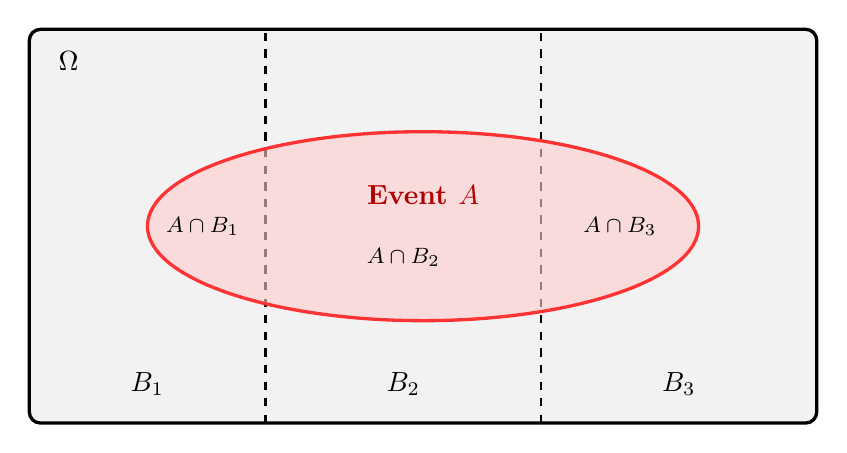
\begin{tikzpicture}[
    thick,
    partition/.style={draw=black!80, fill=blue!5, minimum height=4cm},
    node distance=0cm
]
% Background Sample Space
\draw[rounded corners, fill=gray!10, draw=black, very thick] (-5, -2.5) rectangle (5, 2.5);
\node at (-4.5, 2.1) {\textbf{$\Omega$}};

% Partitions B_i
\draw[dashed] (-2, -2.5) -- (-2, 2.5);
\draw[dashed] (1.5, -2.5) -- (1.5, 2.5);
\node at (-3.5, -2) {$B_1$};
\node at (-0.25, -2) {$B_2$};
\node at (3.25, -2) {$B_3$};

% Event A spanning across partitions
\draw[draw=red!80, fill=red!20, fill opacity=0.6, very thick] 
    (0,0) ellipse (3.5cm and 1.2cm);
\node[text=red!70!black] at (0, 0.4) {\textbf{Event $A$}};

% Intersection labels
\node[font=\footnotesize] at (-2.8, 0) {$A \cap B_1$};
\node[font=\footnotesize] at (-0.25, -0.4) {$A \cap B_2$};
\node[font=\footnotesize] at (2.5, 0) {$A \cap B_3$};

\end{tikzpicture}
\end{center}

\subsection{Pitfalls \& Fallacies}
\begin{itemize}
    \item \textbf{The Overcounting Fallacy:} In committee formation problems, picking $1$ specific type of person first and then picking the rest randomly from the pool double-counts permutations of that group. Always select groups in batch using combinations to preserve uniformity.
    \item \textbf{Confusing Independence with Mutually Exclusive:} Mutually exclusive events ($A \cap B = \emptyset$) are severely \textit{dependent}. If $A$ happens, $B$ cannot. Independent events satisfy $\mathbb{P}(A \cap B) = \mathbb{P}(A)\mathbb{P}(B)$.
\end{itemize}


% ==========================================
% PART 5: CONCEPTUAL SYNTHESIS
% ==========================================
\section{Part 5: Conceptual Synthesis and The "Big Picture"}

\subsection{Thematic Connections}
The central theme unifying this chapter is \textbf{Measure via Isomorphism}. We are learning how to map abstract physical scenarios (e.g., medical patients, auto manufacturing, card games) into rigorous set-theoretic spaces. By establishing a one-to-one correspondence (bijection) between a physical state and a mathematical element $\omega \in \Omega$, we can define a measure $\mathbb{P}$ over the subsets of $\Omega$.

\subsection{Forward and Backward Links}
\begin{itemize}
    \item \textbf{Backward Link:} This extends foundational Set Theory. The algebra of events (unions, intersections, complements) directly parallels Boolean logic (OR, AND, NOT).
    \item \textbf{Forward Link:} Counting measure spaces are the stepping stone to \textit{Lebesgue Integration} and \textit{Continuous Probability Density}. Understanding how a discrete space is partitioned via $\sigma$-algebras is mandatory for mastering Stochastic Calculus, where time-dependent partitions (filtrations) model the flow of information.
\end{itemize}


% ==========================================
% PART 6: ABSTRACT REAL-WORLD MODELING
% ==========================================
\section{Part 6: Abstract Real-World Modeling (Quantitative Finance)}

While combinatorial probability seems discrete, it is the mathematical foundation for the \textbf{Cox-Ross-Rubinstein (CRR) Binomial Options Pricing Model} used by algorithmic traders to price financial derivatives.

\subsection{Model Problem Setup: Binomial Tree Pricing}
Consider a stock with initial price $S_0$. In each discrete time step $\Delta t$, the stock can move up by a factor $u$ or down by a factor $d$, establishing a binary state transition. Over $N$ periods, the sample space of price paths is $\Omega = \{U, D\}^N$.

Let a random path be $\omega = (\omega_1, \dots, \omega_N)$. The number of "up" moves is a random variable $K(\omega) = \sum_{i=1}^N \mathbf{1}_{\{\omega_i = U\}}$. Because the ordering of up and down moves does not affect the terminal price, the terminal stock price only depends on $K$:
\[ S_T = S_0 u^K d^{N-K} \]

By the Fundamental Theorem of Asset Pricing, we must evaluate the derivative under a \textbf{risk-neutral probability measure $\mathbb{Q}$}, where the expected return of the stock is the risk-free rate $r$. The transition probability of an up-move under $\mathbb{Q}$ is strictly defined as $p = \frac{e^{r\Delta t} - d}{u - d}$.

Because the market movements are independent under $\mathbb{Q}$, the measure of any specific path with $k$ up-moves is $p^k (1-p)^{N-k}$. The total number of paths achieving exactly $k$ up-moves is given by the combinatorial formula $\binom{N}{k}$. 

Therefore, to price a European Call Option with strike $X$ and payoff function $\max(S_T - X, 0)$, we compute the expected value of the payoff under $\mathbb{Q}$, discounted back to time zero:
\[ C_0 = e^{-r N \Delta t} \sum_{k=0}^N \binom{N}{k} p^k (1-p)^{N-k} \max(S_0 u^k d^{N-k} - X, 0) \]
This rigorous formula shows how pure combinatorics and event partitioning (Part 2.68) scale directly into multi-billion dollar derivative pricing frameworks.


% ==========================================
% PART 7: COMMON VARIATIONS
% ==========================================
\section{Part 7: Common Variations and Untested Concepts}

An advanced topic missing from the homework is the combination of indistinguishable objects into distinct bins, governed by \textbf{Bose-Einstein Statistics} (commonly called "Stars and Bars").

\begin{theorem}[Stars and Bars]
The number of non-negative integer solutions to the equation $x_1 + x_2 + \dots + x_k = n$ is given by $\binom{n + k - 1}{k - 1}$.
\end{theorem}
\begin{proof}
Consider $n$ identical objects (stars) and $k-1$ partitions (bars). A sequence of stars and bars represents an allocation. For example, for $x_1+x_2+x_3 = 5$, the arrangement $\star \star \mid \star \mid \star \star$ implies $x_1=2, x_2=1, x_3=2$. We have a total of $n + k - 1$ positions. Choosing the locations for the $k-1$ bars uniquely determines the sizes of the $k$ groups. The number of such choices is exactly $\binom{n+k-1}{k-1}$.
\end{proof}


% ==========================================
% PART 8: DIAGNOSTIC TESTING
% ==========================================
\section{Part 8: Advanced Diagnostic Testing: "Find the Flaw"}

Below are 5 advanced proofs/solutions containing a subtle, critical logical flaw. As the grader, attempt to locate the mathematical error.

\begin{enumerate}
    \item \textbf{The Independent Union Flaw:} Let $A$ and $B$ be independent events in a probability space, with $\mathbb{P}(A) = 0.6$ and $\mathbb{P}(B) = 0.5$. We wish to find the probability of their union. Since they are independent, they do not affect each other. Thus, $\mathbb{P}(A \cup B) = \mathbb{P}(A) + \mathbb{P}(B) = 1.1$.
    \item \textbf{The Committee Overcounting Flaw:} A department has 5 female and 7 male professors. We need to form a committee of 3 that contains \textit{at least one} female. Solution: First, pick 1 female to guarantee the requirement ($\binom{5}{1} = 5$ ways). Then pick the remaining 2 committee members from the remaining 11 people ($\binom{11}{2} = 55$ ways). Total ways $= 5 \times 55 = 275$.
    \item \textbf{The Infinite Uniform Measure Flaw:} Consider the sample space of all positive integers $\Omega = \mathbb{Z}^+$. Let $\mathbb{P}$ be a uniform probability measure over this sample space. The probability of choosing any specific integer $k$ is $c$. Since the sum of probabilities must be 1, $\sum_{k=1}^\infty c = 1$.
    \item \textbf{The Base Rate Fallacy:} A machine learning test for a rare disease ($1\%$ prevalence) is $99\%$ accurate (true positive rate = $0.99$, true negative rate = $0.99$). A patient tests positive. The probability the patient actually has the disease is logically $\mathbb{P}(\text{Disease} \mid \text{Positive}) = 0.99$.
    \item \textbf{The Indistinguishable Multinomial Flaw:} We have $n$ identical balls to place into $k$ distinct urns. Since this is an assignment of $n$ items into $k$ groups, we can directly apply the multinomial theorem $\sum \binom{n}{n_1,\dots,n_k}$ to count the number of allocations.
\end{enumerate}

\subsection*{Solution Key to Diagnostic Testing}
\begin{enumerate}
    \item \textbf{Flaw:} Independence is conflated with Mutual Exclusivity. Additivity $\mathbb{P}(A \cup B) = \mathbb{P}(A) + \mathbb{P}(B)$ only applies when $A \cap B = \emptyset$. For independent events, $\mathbb{P}(A \cap B) = \mathbb{P}(A)\mathbb{P}(B) = 0.3$. By Inclusion-Exclusion, $\mathbb{P}(A \cup B) = 0.6 + 0.5 - 0.3 = 0.8$.
    \item \textbf{Flaw:} The proposed method severely overcounts. If women $W_1$ and $W_2$ are selected, picking $W_1$ first and $W_2$ second is treated as a distinct combinatorial path from picking $W_2$ first and $W_1$ second, violating the unordered nature of a committee. Correct method (Complement trick): Total committees - all-male committees = $\binom{12}{3} - \binom{7}{3} = 220 - 35 = 185$.
    \item \textbf{Flaw:} Violation of Kolmogorov's Axioms. A uniform probability measure cannot exist on a countably infinite space. If $c=0$, the sum is $0 \neq 1$. If $c > 0$, the sum diverges to $\infty \neq 1$.
    \item \textbf{Flaw:} Ignoring Bayes' Theorem and the prior probability. Let $D$ be Disease, $P$ be Positive. $\mathbb{P}(D|P) = \frac{\mathbb{P}(P|D)\mathbb{P}(D)}{\mathbb{P}(P)} = \frac{0.99 \times 0.01}{(0.99 \times 0.01) + (0.01 \times 0.99)} = 0.5$. The true probability is only $50\%$.
    \item \textbf{Flaw:} The Multinomial coefficient $\binom{n}{n_1, \dots, n_k}$ assumes the $n$ items are \textit{distinct} (e.g., assigning specific workers to jobs). For \textit{identical} items, Bose-Einstein statistics (Stars and Bars, Part 7) must be used.
\end{enumerate}

\end{document}